%kate: default-dictionary en;

\documentclass[eprint]{actapoly}

\usepackage{algorithm}
\usepackage{algpseudocode}
\usepackage{amssymb}
\usepackage{tikz}
%\usepackage{amsmath, amssymb, amsfonts, amsthm}
%\usepackage{float}
%\usepackage{graphicx}
\usepackage{subcaption}

%\usepackage{draftwatermark}
%\SetWatermarkText{DRAFT}
%\SetWatermarkScale{1}
%\SetWatermarkLightness{0.9}

\begin{document}

%\title[Example of an Article with a Long Title]
%{Example of an Article with a Long Title, the Title Should Be Capitalised 
%Properly in the Code Long Long}
\title[Trajectory Generation Approach]
{Multi Robot Optimal Trajectory Generation}

\author[J. M. Mendes Filho]{Jos\'{e} M. Mendes Filho}{my,their}
\correspondingauthor[E. Lucet]{Eric Lucet}{my}{eric.lucet@cea.fr}

\institution{my}{CEA, LIST, Interactive Robotics Laboratory, Gif-sur-Yvette, 
F-91191, France}
\institution{their}{ENSTA Paristech, Unit\'{e} d'Informatique et d'Ing\'{e}nierie 
des Syst\`{e}mes, 828 bd des Marechaux, 91762, France}
%\institution{their}{ENSTA Paristech, Unit\'{e} informatique et Ingénierie des 
%Système, 828 boulevard des Marechaux, F-91762, France}
%\institution{their}{CEA, LIST, Interactive Robotics Laboratory, 
%Gif-sur-Yvette, F-91191, France}

\begin{abstract}

 This paper proposes the real-time implementation of a multi-robot optimal collision-free motion planner
 algorithm based on a receding horizon approach, for the navigation of a team of mobile
 robots evolving in an industrial context in presence of different structures of obstacles.
 The method is validated in simulation environment for a team of three robots. Then, impact of the algorithm
 parameters setting is studied with regard to critical performance criteria, being mainly real-time implementation,
 obstacle avoidance and time to complete the task.
% In view 
 
\end{abstract}

\keywords{\mbox{multi-robot motion planning}, \mbox{nonholonomic mobile robot}, \mbox{decentralized planning}, \mbox{receding horizon}}

\maketitle




\section{Introduction}\label{sec:intro}




%General Context

The %command and
control of mobile robots is a long-standing subject of research 
in the iterative robotics domain. A trending application of mobile robots systems
is its use in industrial supply-chains for processing orders and optimizing products storage and distribution. Companies such as Amazon and the logistic provider IDEA Groupe employ moble multi-robot systems (Kiva systems, Scallog) for autonomously processing clients orders~\cite{Gizmag,supplychain}.
%such as teams of autonomous forklift trucks
%(for instance Kiva robots used by Amazon~\cite{Gizmag},
%to improve their commercial performance,
Such logistics tasks became increasingly complex as uncertainties sources, such as human presence, are admitted in the work environment.

%Problem

One basic requirement for such mobile robot systems is the capacity of motion planning, i.e., generating admissible configuration and input trajectories that connects two arbitrary states. For solving the motion planning problem, different 
constraints must be taken into account, in particular:

\begin{itemize}

 \item robot's kinematic and dynamic constraints;

 \item geometric constraints;

% \item constraints associated with uncertainties about the current state of 
%world and the outcome of actions.

\end{itemize}

The first constraints derive directly from the mobile robot architecture 
implying in nonholonomic constraints for many types of mobile robots. Geometric 
constraints result from need of preventing the robot to assume specific configurations in order to avoid collisions, communication lost, etc.
% the impossibility of the robots to assume some specific 
%configurations  due to the presence of obstacles, environment bounds, communication range, etc. 
%In turn, uncertainty constraints come from the impossibility of the robots to have an 
%absolute and complete perception of the world (including theirs own states) as 
%well as the outcome of non-stochastic events.


We are particularly interested in solving the problem of planning a 
trajectory for a team of nonholonomic mobile robots in an partially known 
environment occupied by static obstacles being near optimal with respect to the 
execution time (time spent from going from initial to goal configurations).

 

%State of Art

In recent years, a great amount of work towards collision-free trajectory 
planning has been proposed.

 

Some work has been done towards analytic methods for solving the problem for 
certain classes of systems (~\cite{})
TODO cite
. However~\cite{Schwartz1988} shows 
that analytic methods  are inapplicable for nonholonomic systems in presence of 
obstacles.

 

Cell decomposition methods as presented in~\cite{Latombe1991} have the 
downside of requiring a structured configuration space and an \textit{a priori} 
model of its connectivity. Besides, the cell decomposition reduces the space 
of admissible solutions. TODO verify/understand.

 

Initially proposed in~\cite{Khatib1986}, the vector field obstacle avoidance 
method was improve along time for treating problems such as oscillation of the 
solution for narrow passages. This method does not present a near optimal 
generated trajectory.

 

Elastic band approach initially proposed by~\cite{Quinlan1994} and extend to 
mobile manipulators in~\cite{Brock et Khatib, 1998} uses approximations of the 
trajectory shape (combinations of arcs and straight lines) limiting the space 
of solutions and make this method inappropriate for really constrained 
environments.

 

The dynamic window approach~\cite{Fox1997} can handle trajectory 
planning for robots at elevated speeds and in presence of obstacles but is not 
flexible enough to be extended to a multi-robot system.

 

%What do we propose

In this paper, we focus on the development of a motion planning algorithm. 
This algorithm finds collision-free trajectories for a multi-robot system in 
presence of static obstacles which are perceived by the robots as they evolve 
in the environment. The dynamic trajectories found are near optimal with 
respect to the total time spend going from the initial configuration to the 
final one. Besides, this algorithm uses a decentralized approach making the 
system more robust to communication outages and individual robot failure than 
compared to a centralized approach. Identified drawbacks are the dependence on 
several parameters for achieving real-time performance and good solution 
optimality, and not being able to handle dynamic obstacles as it is.

 

This algorithm is based mainly on the work done in~\cite{Defoort2007a} but we 
made changes in particular to respect a precise final configuration for the 
multi-robot system and about how to set parameters for solving the nonlinear 
programming problem (NLP).

 

%Plan

This paper is structured as follows: The second section presents a trajectory 
planning algorithm that solves the problem of one robot going from an initial 
configuration to a final one in the presence of static obstacles. The third 
section extends the method presented in the second section so a collision-free 
trajectory that maintains the communication link between the robots in the 
team can be computed. The forth section is dedicated to the results found by 
this method and the analysis of the computation time and solution quality and 
how they are impacted by the algorithm parameters. The fifth section presents 
the comparison of this approach to another one presented in~\cite{}. Finally, in 
section six we present our conclusions and perspectives.

%\newpage
%\mbox{}\newpage

\section{Problem Statement}\label{sec:problem}

%We consider the following assumptions for the simulation of our approach:
\subsection{Assumptions}
In the development of this approach the following assumptions are made:

\begin{enumerate}

    \item The motion of the multi-robot system begins at
    the instant $t_{init}$ and goes until the instant $t_{final}$.

    \item The team of robots consists of a set $\mathcal{R}$ of $B$
    nonholonomic mobile robots.
    
    \item A robot (denoted $R_b,\ R_b \in \mathcal{R},\ b \in \{0,\dots,B-1\}$) is 
    geometrically represented by a circle of radius $\rho_b$ centered at $(x_b, y_b)$.
        
    \item All obstacles in the environment are considered static. They can be
    represented by a set $\mathcal{O}$ of $M$ static obstacles.
    
    \item An obstacle (denoted $O_m,\ $\mbox{$O_m \in \mathcal{O}$}$,\ $
    \mbox{$m \in \{0,\ \dots, M-1\}$}) is geometrically represented either as
    a circle or as a convex polygon. In the case of a circle its radius is
    denoted $r_{O_m}$ centered at $(x_{O_m},y_{O_m})$.
    
    \item For a given instant $t_k \in [t_{init},\ t_{final}]$, any obstacle
    $O_m$ having its geometric center apart from the geometric center of the
    robot $R_b$ of a distance inferior than the detection radius $d_{b,sen}$
    of the robot $R_b$ is considered detected by this robot.
    Thus, this obstacle is part of the set $\mathcal{O}_b$
    ($\mathcal{O}_b \subset \mathcal{O}$) of detected obstacles.
    
    \item A robot has precise knowledge of the position and geometric representation of
    a detected obstacle.
    
    \item A robot can access 
    information about any robot in the team using 
    a wireless communication link.
    
    \item Latency, communication outages and other problems associated
    to the communication between robots in the team are neglected.
        
    \item Dynamics was neglected.
    
    \item The input of a mobile robot $R_b$ is limited.
    
%    \item The motion planner in a robot $R_b$ (with $n \in {0,\dots,B-1}$) has
%    access to the following information:
%    \begin{enumerate}
%        \item current and past configuration of the robot $R_b$;
%        \item $R_b$'s goal configuration;
%        \item $R_b$'s input limits;
%        \item The map function to pass from flat space to state and input space and
%        its inverse;
%        \item  
%    \end{enumerate}

%     as well as the its robot's goal configuration, the input limits,
%    its kinematic
%    model and bijective mapping function for passing from the flat space to the
%    actual state and input spaces;
%    
%    \item Each robot have sensors that can detect the surrounding region within a
%    radius $\rho_d$. Any object having its geometric center within this region is
%    considered detect by the robot;

\end{enumerate}

\subsection{Constraints and cost functions}

After loosely defining what is the motion planning problem in
Section~\ref{sec:intro} and presenting the assumptions in the previous Subsection
we can identify and define what are the constraints and the cost function for the
multi-robot navigation.

\begin{enumerate}

    \item The solution of the motion planning problem
    for the robot $R_b$ represented by the pair
    $(q^{*}_b(t), u^{*}_b(t))$ --
    $q^{*}_b(t) \in \mathbb{R}^n$ being the solution trajectory for
    the robot's configuration and $u^{*}_b(t) \in \mathbb{R}^p$ the solution
    trajectory for the robot's input -- must satisfy the
    robots kinematic model equation:   
%    For a robot $R_b$     
%    its kinematic model equation
%    must hold for a computed solution to the
%    motion planning problem:
    \begin{equation}
        \dot{q}^{*}_b(t) = f(q^{*}_b(t),u^{*}_b(t)),\quad \forall t \in [t_{init}, t_{final}].
    \end{equation}
%	with $q^{*}_b(t) \in \mathbb{R}^n$ the solution 
%	trajectory for the robot's configuration,
%	$u^{*}_b(t) \in \mathbb{R}^p$ the solution trajectory
%	for the robot's input and
%	\mbox{$f\,:\,\mathbb{R}^{n}\times \mathbb{R}^{p}\rightarrow \mathbb{R}^n$} the
%	vector-valued function modelling the robot 
%	kinematics.
    
    \item The planned initial configuration and initial 
    input for the robot $R_b$ must
    be equal to the initial configuration and initial
    input of $R_b$:
    \begin{equation}
        q^{*}_{b}(t_{init}) = q_{b,init},
    \end{equation}
    \begin{equation}
        u^{*}_{b}(t_{init}) = u_{b,init}.
    \end{equation}

    \item The planned final configuration and final 
    input for the robot $R_b$ must
    be equal to the goal configuration and goal
    input for $R_b$:
    \begin{equation}\label{eq:finalconfig}
        q^{*}_{b}(t_{final}) = q_{b,goal},
    \end{equation}
    \begin{equation}\label{eq:finalinput}
        u^{*}_{b}(t_{final}) = u_{b,goal}.
    \end{equation}

    \item The practical limitations of the input impose
    the following constraint: $\forall t \in [t_{init}, t_{final}]$, $\forall i \in [1,2,\cdots, p]$,
    \begin{equation}
        |u^{*}_{b,i}(t)| \leq u_{b,i,max}.
    \end{equation}
    
    \item The cost for the multi-robot system navigation is defined as:
    \begin{equation}
        L(q(t),u(t)) = \sum_{b=0}^{B-1}L_b(q_b(t), u_b(t), q_{b,goal},u_{b,goal})
    \end{equation}
    where $L_b(q_b(t), u_b(t), q_{b,goal},u_{b,goal})$ is the 
    integrated cost for one robot
    motion planning (see~\cite{Defoort2009}).
    
    \item 
    %TODO define the functions "distance" robot-to-obstacle:
    To ensure collision avoidance with obstacles the euclidean 
    distance between
    a robot and an obstacle (denoted $\mathrm{d}(R_b, O_m)\ |\ O_m
    \in \mathcal{O}_b, R_b \in \mathcal{B} $) has to satisfy:
    \begin{equation}
    	\mathrm{d}(R_b, O_m) \geq 0.
    \end{equation}
    
    For the circle representation of an obstacle the distance
    $\mathrm{d}(R_b, O_m)$ is defined as:
    \begin{equation*}
        \sqrt{(x_{b} - x_{O_m})^2 + (y_{b} - y_{\mathrm{O}_m})^2}  - \rho_b - r_{O_m}.
    \end{equation*}
    
    For the polygon representation, the distance was calculated using three different
    definitions according to the Voronoi region~\cite{ericson2004real}
    $R_b$ is located. Figure~\ref{fig:convexpolygon} shows an example of the three kinds
    of regions for a quadrilateral $ABCD$ representation. The Voronoi regions are 
    defined by
    the lines containing the sides ($s$ lines) and by the lines passing
    through the vertices that are orthogonal to the sides ($r$ lines).    
    
	In this example, the region in which the robot $R_b$ is located
	at an instant $t_k$
	can be computed by evaluating the line
 	equations 
 	$s_{AB}$, $s_{BC}$, $s_{CD}$, $s_{DA}$, $r_{AB}$, $r_{AD}$, $r_{BA}$, $r_{BA}$,
 	$r_{BC}$, $r_{BA}$, $r_{BC}$, $r_{CB}$, $r_{CD}$, $r_{DC}$ and $r_{DA}$ for 
 	the position associated with the configuration $q^*_b(t_k)$.
 	
%    The region which the position associated with a given configuration $q_b$
%    is in can be computed as follows.

    TODO: for the quadrilateral we have 9 regions, the 3 that shown...
    
    In addition, the distance
    robot-to-quadrilateral could be found as follows:
    \begin{enumerate}
    
	   	\item If robot in region $1$:
   	   	\begin{equation*}
    	    \sqrt{(x_{b} - x_{A})^2 + (y_{b} - y_{A})^2} - \rho_b
	    \end{equation*}
	    which is simply the distance of the robot to the vertex $A$.
	    
	    \item If robot in region $2$:
%	    
		\begin{equation*}
			\mathrm{d}(s_{DA}, (x_{b}, y_{b})) - \rho_b
		\end{equation*}
		where
   	   	\begin{equation*}
    	    \mathrm{d}(s_{DA}, (x_{b}, y_{b})) =\\ \frac{|a_{s_{DA}}x_{b} + b_{s_{DA}}y_{b}
    	    + c_{s_{DA}}|}{\sqrt{a_{s_{DA}}^2 + b_{s_{DA}}^2}}.
	    \end{equation*}
	    
	    The distance $\mathrm{d}(s_{DA}, (x_{b}, y_{b}))$ represents the distance from the robot to the side $DA$.
	    
	    \item If robot in region $3$:
   	   	\begin{equation*}
    	    -\min\left(\mathrm{d}(s_{AB}, (x_{b}, y_{b})), \cdots, \mathrm{d}(s_{DA}, (x_{b}, y_{b}))\right) - \rho_b
	    \end{equation*}
	    which represents the amount of penetration of the robot in the obstacle.
	    
    \end{enumerate}
    
    
    \begin{figure}[!h]
	\centering
	{
	    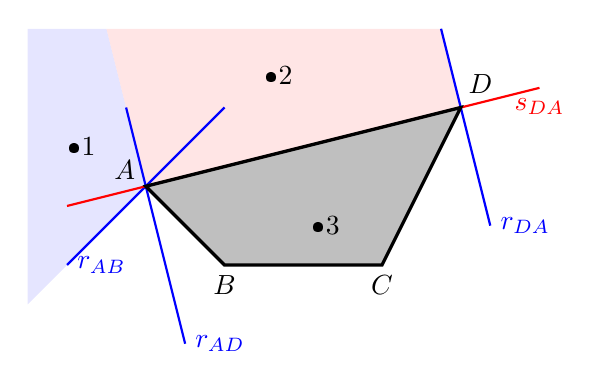
\begin{tikzpicture}
		[polygon/.style={very thick, black},
		axis/.style={-,blue,thick},
		point/.style={very thick,black},
		afill/.style = {fill=blue!20,fill opacity=0.5},
		bfill/.style = {fill=red!20,fill opacity=0.5}]
		
		\fill[afill] (0,1,0) -- (-0.5,3,0) -- (-1.5,3,0) -- (-1.5,-.5,0) --cycle;
		\fill[bfill] (0,1,0) -- (4,2,0) -- (3.75,3.,0) -- (-0.5,3,0) --cycle;
		
		\draw[axis] (-.25,2.,0) -- (.5,-1.,0) node[anchor=west,color=blue]
		{$r_{AD}$}; % y = 1. - 4.x
		
		\draw[axis] (1.,2.,0) -- (-1.,0.,0) node[anchor=west,color=blue]
		{$r_{AB}$};%y = x+1
	
		\draw[axis] (3.75,3.,0) -- (4.375,0.5,0) node[anchor=west,color=blue]
		{$r_{DA}$}; %y = 18.-4. x
	
		\draw[axis,red] (-1.,.75,0) -- (5.,2.25,0) node[anchor=north,color=red]
		{$s_{DA}$};
		
		\draw[polygon,fill=gray!50] (0,1,0)  -- (1,0,0) node[below] {$B$}
		-- (3,0,0) node[below] {$C$} -- (4,2,0) -- cycle;
		\node[text width=0cm] at (-0.4,1.2,0) {$A$};
		\node[text width=0cm] at (4.1,2.3,0) {$D$};
			
		\draw[point] (2.0,2.4,0) node[anchor=east]{\textbullet $2$};
		\draw[point] (-0.5,1.5,0) node[anchor=east]{\textbullet $1$};
		\draw[point] (2.6,0.5,0) node[anchor=east]{\textbullet $3$};
	
		\end{tikzpicture}}
	\caption{Voronoi regions used for case differentiation. \label{fig:convexpolygon}}
	\end{figure}

    \item 
    In order to prevent inter-robot collisions the following constraint must be respected:
    $\forall\ (R_b, R_c) \in \mathcal{R} \times \mathcal{R}, b\neq c, c \in \mathcal{C}_b$,
    %o a robot $R_b$ avoid collision with other robots the following
    %relation must be satisfied. 
%    In order to avoid inter-robot collision the following constraint
%    must be respect by the robots $R_b$ and $R_b$:
    \begin{equation}\label{eq:coll}
	    \mathrm{d}(R_b,R_c) - \rho_b -\rho_c \geq 0
    \end{equation}
    where $\mathrm{d}(R_b,R_c) = \sqrt{(x_{b} - x_{c})^2 + (y_{b} - y_{c})^2}$ and
    $\mathcal{C}_b$ is the set of robots that present a collision risk with
    $R_b$.
%    This constraint justifies the need for a communication link between the robots.
    
    \item Finally, the need of a communication link between two robots $(R_b, R_c)$ yields to
    the following constraint:
    %In addition, for a given pair of robots $R_b R_c$ that must keep
    %a communication link between them the following equation 
    \begin{equation}\label{eq:com}
    	\mathrm{d}(R_b,R_c)  - \min(d_{b,com}, d_{c,com}) \leq 0
    \end{equation}
    with $d_{b,com}, d_{c,com}$ the communication link reach of each robot and
    $\mathcal{D}_b$ is the set of robots that present a communication lost risk with
    $R_b$.
\end{enumerate}
%\newpage
%\mbox{}\newpage



\section{Distributed motion planning}



\subsection{Receding horizon approach}\label{subsec:rha}

%Defoort give in \cite{    Defoort2007a} an example showing how a unicycle model 
%can be written using the flatness property.
%The basis algorithm for planning for a mono robot is based on the optimization 
%problem shown in equations~\ref{eq:} and~\ref{eq:}.
%TODO present method or make reference to Defoort introducing $T_c$, $T_p$ etc.

As said before trying to find the solution from the initial configuration
until the goal is not feasible. Thus, the planning has to be computed on-line
as the multi-robot system evolves in the environment.
One way to do so is to use a receding horizon control approach~\cite{Keviczky2006}.


All robots in the team use the same constant planning horizon $T_p$ and update
horizon $T_c$. $T_p$ is the time horizon for which a solution will be computed,
$T_c$ is the time horizon during which a plan is be execute while the
next plan, for the next timespan $T_p$, is being computed.


For each receding horizon planning problem the following is done:
\paragraph{Step 1.}\label{step1} Compute an intended solution trajectory (denoted $(\hat{q}_b(t), \hat{u}_b(t))$)
by ignoring coupling
constraints, i. e., constraints \ref{eq:coll} and \ref{eq:com} that involve other
robots in the team.
\paragraph{Step 2.}\label{step2} Robots involved in a conflict (collision or lost of communication)
update their trajectories
by solving another constrained optimization problem that take into account
coupling constraints (\ref{eq:coll} and \ref{eq:com}).
This is done by using the other robots' intended
trajectories computed in the previous step as an estimative of the robots
final trajectories. If a robot is not involved in any conflict its final
solution trajectory is identical to the one estimated in the \nameref{step1}.

\mbox{}

This scheme is explained in details in~\cite{Defoort2007a} where the receding horizon optimization
problems are formulated based on the constraints and cost function defined in Section~\ref{sec:problem}.

However, constraints related to the goal configuration and input of the motion planning problem are
neglected in the receding horizon scheme presented in~\cite{Defoort2007a}.
The constraints~\ref{eq:finalconfig} and~\ref{eq:finalinput} are not considered
in the receding horizon optimization problems.
For that, a termination procedure is proposed in the following that enables the robots to reach their
goal state.


\subsection{Motion planning termination}


As the robots evolve theirs states approximate to the goal states.
%That is the  since the distance between current and final state is what is to 
%be minimized.
But simply stopping the motion planner as the robots are in the neighbourhood of
their final configuration is not a satisfying approach (it leaves 
constraints~\ref{eq:finalconfig} and~\ref{eq:finalinput} unsatisfied).

%Furthermore, the use of a constant planning horizon $T_p$ prevents the robot of
%finding 

By considering those constraints in the termination optimization problem and by planning for
an undetermined planning horizon the goal configuration can be reached.

%The constraints associated to the final configuration and input have to be integrated 
%into the optimization problem. In addition, the timespan for performing this last
%termination plan cannot be constant and must be one of the values to be calculated.
%The fixed planning horizon has to be made variable in order to get to the 

The criterion used to pass from the receding horizon optimization problem to the termination optimization problem
is define below in the equation~\ref{eq:stopcond}:

\begin{align}\label{eq:stopcond}
  d_{rem} \geq d_{min} + T_c \cdot v_{max}
\end{align}

This equation insures that the termination plan will be planned for at least a 
$d_{min}$ distance from the robot's goal position.
This minimal distance is assumed to be sufficient for the robot to reach the 
goal configuration.

After stopping the receding horizon planning we calculate new parameters for the 
solution representation and computation taking into
account the estimate remaining distance and the typical distance travelled
for a $T_d$ planning horizon (for instance, the discretization of the time).

The following pseudo code~\ref{cod:algo} summarizes the planning algorithm
and the Figure~\ref{fig:recedinghor} illustrates its results.

In the pseudo code we see the call of a {\scshape PlanSec} procedure.
It represents the resolution of the of the receding horizon planning problem
as defined in subsection~\ref{subsec:rha}.

{\scshape PlanLastSec} is the procedure that solves the termination planning
problem. This problem is similar to the receding horizon planning problems.
It also has the two steps presented before for computing an intended plan and
for updating it, if need be, so conflicts (collision and communication lost)
are avoided. The difference consists in how the optimization problems associated
are defined. The optimization problem defined in equations \ref{eq:costsa} and
\ref{eq:constsa} is the problem solved at the first step which generates an
intended plan (denoted ($\hat{q}_b(t)$, $\hat{u}_b(t)$)). The optimization
problem associated with the update step is defined in equations 
\ref{eq:cost} and \ref{eq:const} and produces the final solution ($q^*_b(t)$, $u^*_b(t)$).

In these new optimal problems the planning horizon is not a constant as before, instead it is a part of the solution to be found.

\begin{algorithm}
    \caption{Motion planning algorithm\label{cod:algo}}
    \label{swpa}
    \begin{algorithmic}[1] % The number tells where the line numbering should start
        \Procedure{Plan}{} %\Comment{The g.c.d. of a and b}
%	    \State $knots \gets $\Call{GenKnots}{$t_p,d_{spl},n_{knots}$}
%	    \State $time \gets $\Call{LineSpacing}{$0,t_p,n_{s}$}
	    %\State $z_{latest} \gets $\Call{$\varphi_0$}{$q_{initial}$}
	    \State $q_{latest} \gets q_{initial}$
	    %\State $ctrlpts \gets $\Call {InitCtrlPts}{$q_{initial},q_{final},T_p,u_{max}$}
	    %\State \Call{Init}{}
	    \State $d_{rem} \gets |${\scshape Pos}$(q_{final}) - ${\scshape Pos}$(q_{latest})|$
	    \While{$d_{rem} \geq d_{min} + T_c \cdot v_{max}$}
	    \State \Call{InitSolRepresentation}{$\cdots$}
		\State $q_{latest} \gets $\Call{PlanSec}{$\cdots$}
		\State $d_{rem} \gets |${\scshape Pos}$(q_{final}) - ${\scshape Pos}$(q_{latest})|$
		
	    \EndWhile\label{planningwhile}
	    \State \Call{RescaleRepresentation}{$\cdots$}
%	    \State $s \gets $\Call {Min}{$\tfrac{d_{rem}}{v_{max}\cdot t_p}, 1.0$}
%	    \State $n_{knots} \gets $\Call{Max}{\Call{Round}{$s\cdot n_{knots}$}$, d_{spl}$}
%	    \State $n_{s} \gets $\Call {Max}{\Call{Round}{$s\cdot n_{s}$}$, n_{knots} + d_{spl}$}
	    \State $T_f \gets $\Call{PlanLastSec}{$\cdots$}
	    
%            \State $r\gets a \bmod b$
%            \While{$r\not=0$} %\Comment{We have the answer if r is 0
%                \State $a \gets b$
%                \State $b \gets r$
%                \State $r \gets a \bmod b$
%            \EndWhile\label{euclidendwhile}
%            \State \textbf{return} $b$%\Comment{The gcd is b}
        \EndProcedure
    \end{algorithmic}
\end{algorithm}

\begin{figure}[!h]
  \centering
  \includegraphics[width=\linewidth]{./images/receding_horizon/motionplanning2.png} %
  %\rule{5cm}{5cm} % <-- this is just a black box substitute for graphics
  \caption{Receding horizon scheme with termination plan. The timespan $T_f$ represents the duration of the plan for reaching the goal configuration.\label{fig:recedinghor}}
\end{figure}

\begin{align}\label{eq:costsa}
\underset{\hat{q}_b(t),\hat{u}_b(t),T_f}{\mathrm{min}} L_{b,f}(\hat{q}_b(t), \hat{u}_b(t), q_{b,goal},u_{b,goal})
\end{align}

under the following constraints for $\tau_k = kT_c$ with $k$ the number of receding horizon
problems solved before the termination problem:
\begin{equation}\label{eq:constsa}
\left\lbrace\begin{array}{lcl}
    \dot{\hat{q}}_b(t) = f(\hat{q}_b(t),\hat{u}_b(t)),\ \ \forall t \in [\tau_{k}, \tau_{k}+T_f]\\
    \hat{q}_b(\tau_{k}) = q^*_{b}(\tau_{k-1}+T_c)\\
    \hat{u}_b(\tau_{k}) = u^*_{b}(\tau_{k-1}+T_c)\\
    \hat{q}_b(\tau_{k}+T_f) = q_{b,goal}\\
    \hat{u}_b(\tau_{k}+T_f) = u_{b,goal}\\
    |\hat{u}_{b,i}(t)| \leq u_{b,i,max},\ \ \forall i \in [1,p],\forall t \in (\tau_{k}, \tau_{k}+T_f)\\
    d(R_b, O_m) \geq 0,\quad \forall O_m \in \mathcal{O}_b, t \in (\tau_{k}, \tau_{k}+T_f)
\end{array}\right.
\end{equation}

\begin{align}\label{eq:cost}
\underset{q^*_b(t),u^*_b(t),T_f}{\mathrm{min}} L_{b,f}(q^*_b(t), u^*_b(t), q_{b,goal},u_{b,goal})
\end{align}

under the following constraints:
\begin{equation}\label{eq:const}
\left\lbrace\begin{array}{lcl}
    \dot{q^*}_b(t) = f(q^*_b(t),u^*_b(t)),\ \ \forall t \in [\tau_{k}, \tau_{k}+T_f]\\
    q^*_b(\tau_{k}) = q^*_{b}(\tau_{k-1}+T_c)\\
    u^*_b(\tau_{k}) = u^*_{b}(\tau_{k-1}+T_c)\\
    q^*_b(\tau_{k}+T_f) = q_{b,goal}\\
    u^*_b(\tau_{k}+T_f) = u_{b,goal}\\
    |u^*_{b,i}(t)| \leq u_{b,i,max},\ \ \forall i \in [1,p],\forall t \in (\tau_{k}, \tau_{k}+T_f)\\
    d(R_b, O_m) \geq 0,\ \ \forall O_m \in \mathcal{O}_b, \forall t \in (\tau_{k}, \tau_{k}+T_f)\\
    \mathrm{d}(R_b, R_c) - \rho_b - \rho_c \geq 0,\ \ \forall R_c \in \mathcal{C}_b, \forall t \in (\tau_{k}, \tau_{k}+T_f)\\
    \mathrm{d}(R_b, R_d) - \min(d_{b,com},d_{d,com}) \geq 0,\ \ \forall R_d \in \mathcal{D}_b,\\
    \quad \quad \quad \quad \quad \quad \quad \quad \quad \quad \quad \quad \quad \quad \quad \forall t \in (\tau_{k}, \tau_{k}+T_f)\\
    \mathrm{d}(q^*_b(t), \hat{q}_b(t)) \leq \xi,\ \ \forall t \in (\tau_{k}, \tau_{k}+T_f)
\end{array}\right.
\end{equation}

A possible definition for the $L_{b,f}$ cost function can be simply $T_f$.
The sets $\mathcal{O}_b$, $\mathcal{C}_b$ and $\mathcal{D}_b$ are functions of
$\tau_k$.




\subsection{Strategies for solving the constrained optimization problems}



\subsubsection{Flatness property}

As explained in~\cite{Defoort2007a} all mobile robots consisting of a solid
block in motion can be modelled as a flat system. 
This means that a change of variables is possible in a way that states and
inputs of the kinematic model of the mobile robot can be written in terms
of the new variable, called flat output ($z$), and its $l$th first derivatives.
Thus, the behaviour of the system can be completely determined by the flat
output.

%\begin{figure}[!h]\centering
%  \includegraphics[width=.7\linewidth]{./images/flatness.png} %
%  \caption{Flatness\label{fig:flatness}}
%\label{fig:res}
%\end{figure}

Searching for a solution to our problem in the flat space rather than in
the actual configuration space of the system present advantages.
It prevents the need for integrating the differential equations
of system and reduces the dimension of the problem of finding an optimal
admissible trajectory.
After finding (optimal) trajectories in the flat space it is possible
to retrieve back the original configuration and input trajectories.
%as shown in Figure~\ref{fig:flatness}.

\subsubsection{Parametrization of the flat output by B-splines}

Another important aspect of this approach is the parametrization of 
the flat output trajectory. As done done in~\cite{milam2003} the use
of B-spline functions present interesting properties:


\begin{itemize}


 \item It is possible to specify a level of continuity $C^k$ when using
 B-splines without additional constraints.
 
 \item B-spline presents a local support, i.e., changes in parameters values have a local
 impact on the resulting curve.
 
 
\end{itemize}

The first property is very well suited for parametrizing the flat output since
its $l$th first derivatives will be needed when computing the system actual state
and input trajectories. The second property is important when searching for an
admissible solution in the flat space; such parametrization is more efficient
and well-conditioned than, for instance, a polynomial parametrization.

TODO cite

\subsubsection{Optimization solver}

There is a variety of numerical optimization packages implemented in many different programming languages available for solving optimization problems~\cite{pyopt-paper}.

Obviously not all of those implementations are suited for solving
the particular kind of optimization problems presented before.

As explained in~\ref{Defoort2009} a Feasible Sequential Quadratic Programming is best suited for solving the motion
planning problem as stated in thins paper. 
This class of solvers compute at every iteration solution
that respects the problem constraints.

TODO keep explaining, present SLSQL and ALGENCAN, present reasons why we used SLSQP (i.e. availability in python, free license, and faster then ALGENCAN)

\paragraph{SLSQP numerical stability}

%\newpage
%\mbox{}\newpage




\section{Simulation results}

Here we show the results and analyses founded for the motion planner presented
in the previous sections.

The trajectory and velocities shown in the Figures~\ref{fig:collision} and~\ref{fig:nocollision}
illustrate a motion planning solution found for a team of three robots.
The robots move in an environment where three static obstacles are present.
Each point along the trajectory line of a robot represents the beginning
of a $Tc$ computation horizon.

In Figure~\ref{fig:collision} we show the resulting plan when coupling constraints
are ignored (\nameref{step2} is never performed). In Figure~\ref{fig:nocollision}
we have a collision-free solution. The blue zones in Figure~\ref{fig:nocollision} are in the same position as the red ones in Figure~\ref{fig:collision}. Specially near these regions a change in the trajectory is present. Complementary, changes in the robots velocities across charts in both figures can be notice. Finally, the bottom charts show that the collisions were indeed avoid: inter-robot distances in Figure~\ref{fig:nocollision} are greater then or equal to zero all along the simulation.
%The trajectories and
%velocities resulting from the solution update.

%TODO distance robot-to-robot for the 2 cases

\begin{figure}[!h]\centering
  \includegraphics[width=\linewidth]{./images/collision/multirobot-path.pdf} %
  %\rule{5cm}{5cm} % <-- this is just a black box substitute for graphics
  \\[1mm]
  \includegraphics[width=\linewidth]{./images/collision/multirobot-vw.pdf} % 
  %\rule{5cm}{5cm} % <-- this is just a black box substitute for graphics
  \includegraphics[width=\linewidth]{./images/collision/multirobot-interr.pdf} % 
  %\rule{5cm}{5cm} % <-- this is just a black box substitute for graphics
  \caption{Motion planning solution without collision handling\label{fig:collision}}
\label{fig:res}
\end{figure}

\begin{figure}\centering
  \includegraphics[width=\linewidth]{./images/no_collision/multirobot-path2.pdf} 
% <-- use this for your graphics
  %\rule{5cm}{5cm} % <-- this is just a black box substitute for graphics
  \\[1mm]
  \includegraphics[width=\linewidth]{./images/no_collision/multirobot-vw.pdf} %
  %\rule{5cm}{5cm} % <-- this is just a black box substitute for graphics
  \includegraphics[width=\linewidth]{./images/no_collision/multirobot-interr.pdf} %
  %\rule{5cm}{5cm} % <-- this is just a black box substitute for graphics
  \caption{Motion planning solution with collision handling\label{fig:nocollision}}
\label{fig:res}
\end{figure}

For performing these two previous simulations a reasonable number of parameters have to be set. These parameters can be categorized into two groups. The \textbf{algorithm related} parameters and the \textbf{optimization solver related} ones.
Among the former group, the most important ones are:
\begin{itemize}
\item[$\bullet$] The number of sample for time discretization ($N_s$);
\item[$\bullet$] The number of internal knots for the B-splines curves ($n_{knots}$);
\item[$\bullet$] The planning horizon for the sliding window ($T_p$);
\item[$\bullet$] The computation horizon ($T_c$).
\end{itemize}

The latter kind depends on the numeric optimization solver adopted.
However, since most of them are iterative methods, it is common
to have at least the two following parameters:
\begin{itemize}
\item[$\bullet$] Maximum number of iterations;
\item[$\bullet$] Stop condition.
\end{itemize}

%The task of searching for a satisfactory set of parameters' values with regard to a performance metric (e.g. total time to complete the miss1ion) is quite laborious.

This considerable number of parameters having influence on the solution
and/or on the time for finding a solution makes the search for a
satisfactory set of parameters' values a laborious task.

Thus, it is important to have a better understanding of how some
performance criteria are impacted by the changes in algorithm
parameters.

\subsection{Parameters' impact analyses}

Three criteria considered important for the validation of this method were studied.
We tested different parameters configuration and scenario in order to 
understand how they influence
those criteria.
The three criteria defined for a given robot $R_b$ are:

\begin{itemize}

\item
\textit{Maximum computation time} over the computation horizon ($MCT/T_c$ 
ratio).

\item
Obstacle penetration area ($P$).

\item
Total execution time ($T_{tot}$).

\end{itemize}

\subsubsection{Detection radius impact}

As the detection radius of the robot increases more obstacles are
seen at once which, in turn,
increases the number of constraints in the optimization problems.
The impact of increasing the detection radius $d_{b,sen}$ in the computation
performance (\textit{Maximum computation time} over computation horizon $MCT/T_c$) can
be seen in the Figure~\ref{fig:drhormp} for a scenario where seven obstacles where present.
Naturally, the computation time stops increasing as the robot sees all obstacles present
in the environment.

\begin{figure}[!h]\centering
  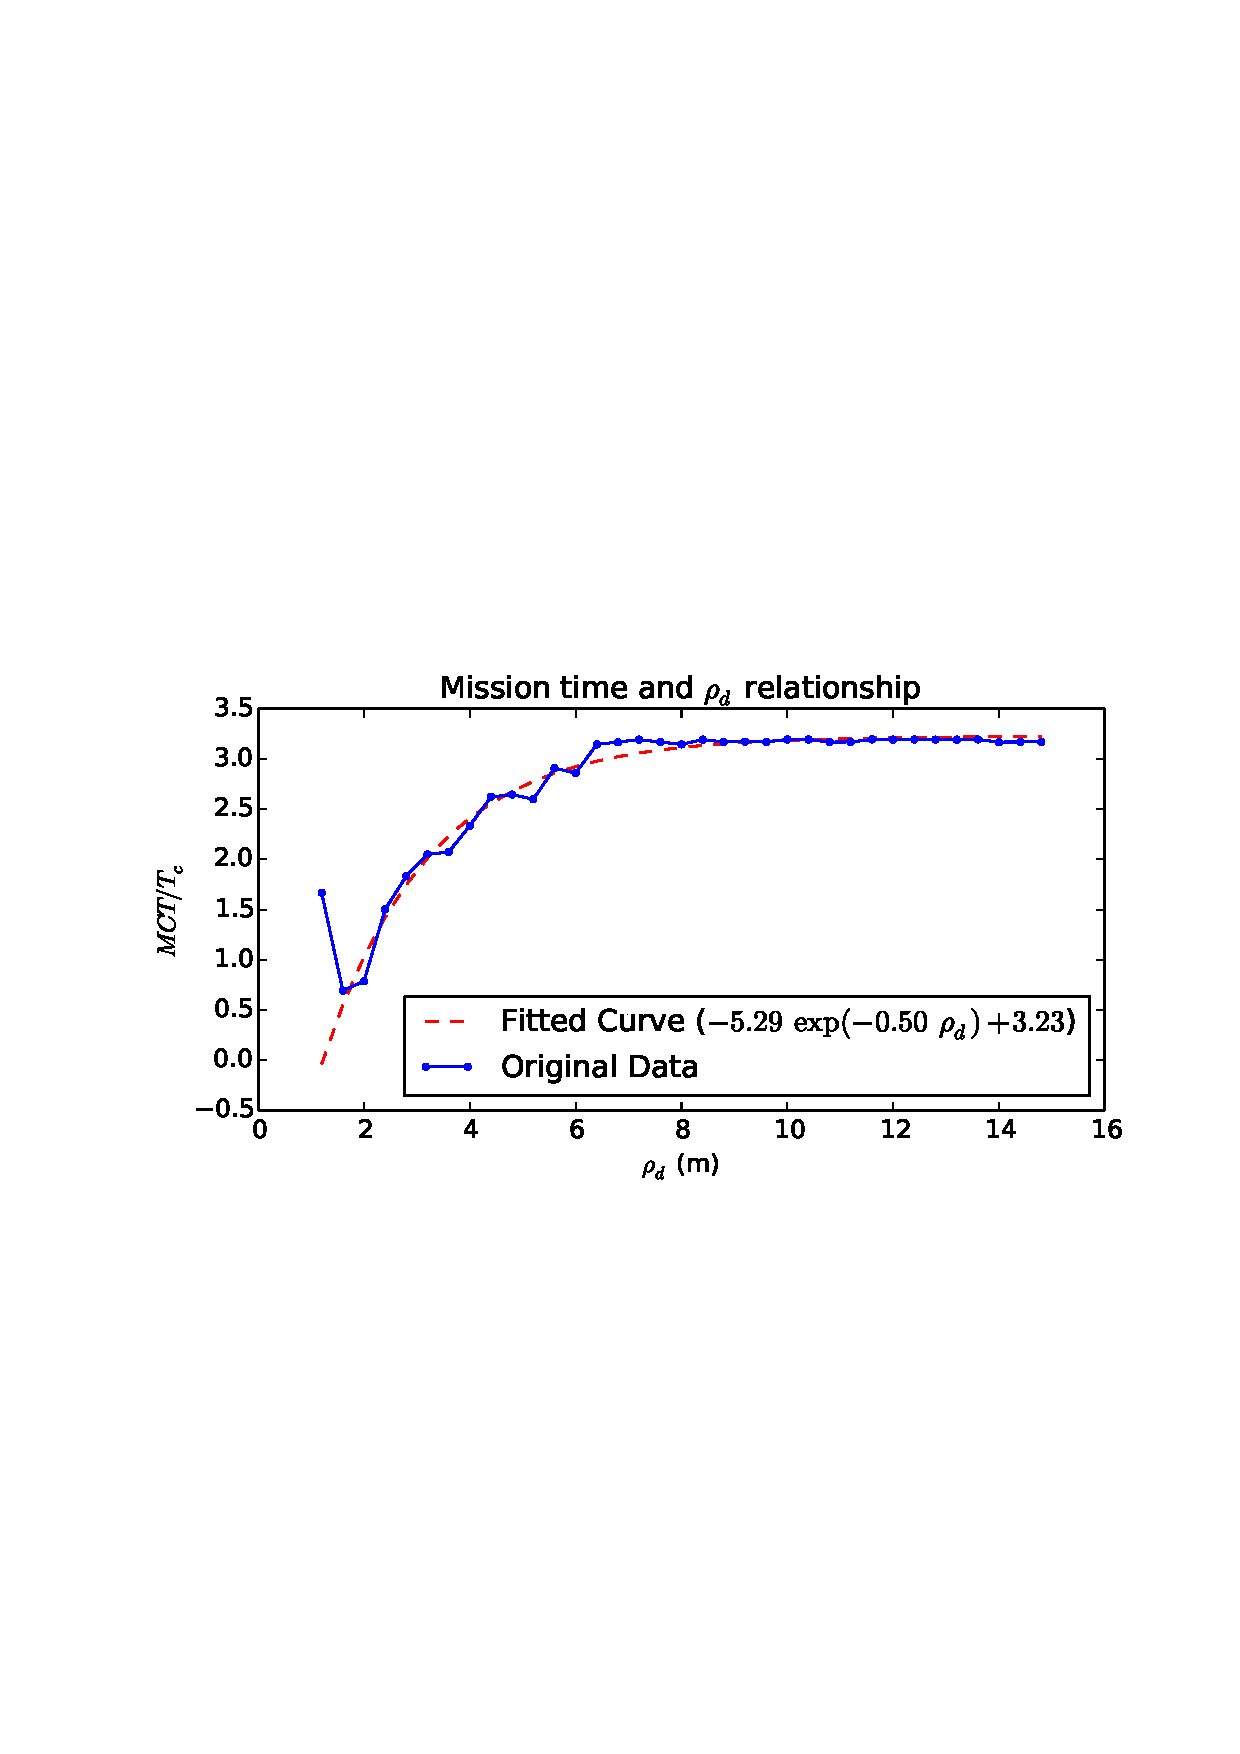
\includegraphics[width=\linewidth]{./images/drho/drho-rmp.pdf} % <-- use this
  %\rule{5cm}{5cm} % <-- this is just a black box substitute for graphics
  \caption{Increasing of detection radius and impact on a $MTC/T_c$ 
ratio\label{fig:drhormp}}
\end{figure}

Furthermore, the Figure~\ref{fig:drhotot} shows how the total time of execution
decreases as the radius increases pointing out how a better knowledge of the
environment produces a more optimal solution.

%As the detection radius of the robot increases more obstacles are
%seen at a time which, in turn,
%increases the number of constraints in the optimization problems.
%The impact of increasing the detection radius $d_{b,sen}$ in the computation
%performance (\textit{Maximum computation time} over computation horizon $MCT/T_c$) can
%be seen in the Figure~\ref{fig:drho}.

\begin{figure}[!h]\centering
  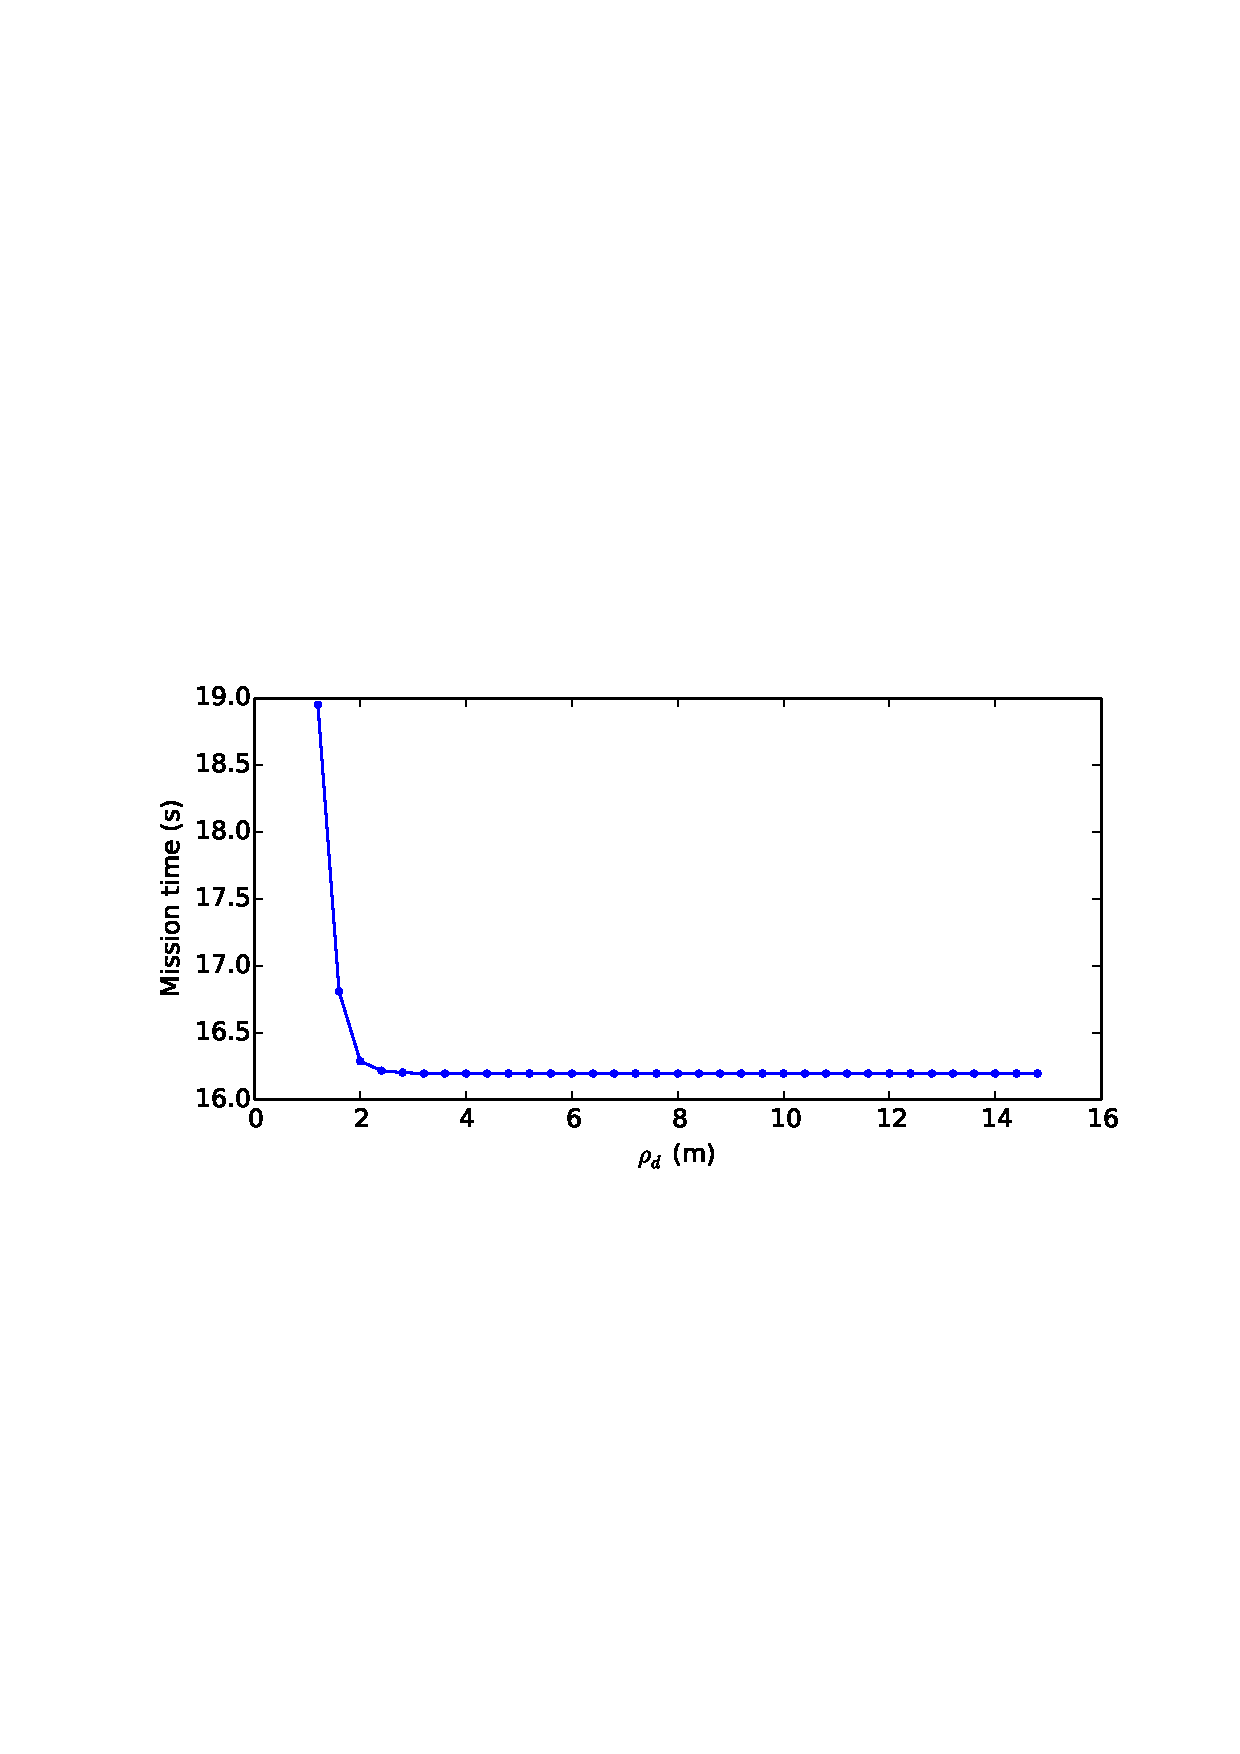
\includegraphics[width=\linewidth]{./images/drho/drho-tot.pdf}
  \caption{Increasing of detection radius and impact on a $T_{tot}$ 
ratio\label{fig:drhotot}}
\end{figure}

These two behaviors indicate how a compromise between computation time and optimality must be found.

%The numbers that can be seen
%over the blue curve are the maximum number of obstacles seen at once during the whole mission.

\subsection{Maximum computation time over computation horizon $MCT/T_c$}

The significance of this criterion lays in the need of assuring the 
real-time property of this algorithm.
In a real implementation of this approach the computation horizon would have 
always to be superior than the
maximum time took for computing a plan (coupling constraints
taken into account).

Based on several simulations with different scenarios we were able to
produce the charts shown in the Figure~\ref{fig:uni3}

\begin{figure}[!h]
        \centering
        ~ %add desired spacing between images, e. g. ~, \quad, \qquad, \hfill etc.
          %(or a blank line to force the subfigure onto a new line)
        \begin{subfigure}[b]{0.48\textwidth}
                \includegraphics[width=\textwidth]{./images/realtime/Scenario_3__N_knots_4/mcttc-tctp.eps}
                \caption{Four internal knots. Average variance between lines is $1.047\times 10^{-2}$}\label{fig:uni34}
        \end{subfigure}
        
        ~ %add desired spacing between images, e. g. ~, \quad, \qquad, \hfill etc.
          %(or a blank line to force the subfigure onto a new line)
        \begin{subfigure}[b]{0.48\textwidth}
                \includegraphics[width=\textwidth]{./images/realtime/Scenario_3__N_knots_5/mcttc-tctp.eps}
                \caption{Five internal knots. Average variance between lines is $0.972\times 10^{-2}$}\label{fig:uni35}
        \end{subfigure}
        ~ %add desired spacing between images, e. g. ~, \quad, \qquad, \hfill etc.
          %(or a blank line to force the subfigure onto a new line)
        \begin{subfigure}[b]{0.48\textwidth}
                \includegraphics[width=\textwidth]{./images/realtime/Scenario_3__N_knots_6/mcttc-tctp.eps}
                \caption{Six internal knots. Average variance between lines is $0.587\times 10^{-2}$}\label{fig:uni36}
        \end{subfigure}
        \caption{Three obstacles scenario}\label{fig:uni3}
\end{figure}

\begin{itemize}
 \item 
 SLSPQ method request $O(n^3)$ time, $n$ being the number of knots; 
\end{itemize}

\subsection{Obstacle penetration $P$}

\ref{fig:pen}
TODO rescale images

\begin{figure}[!h]\centering
  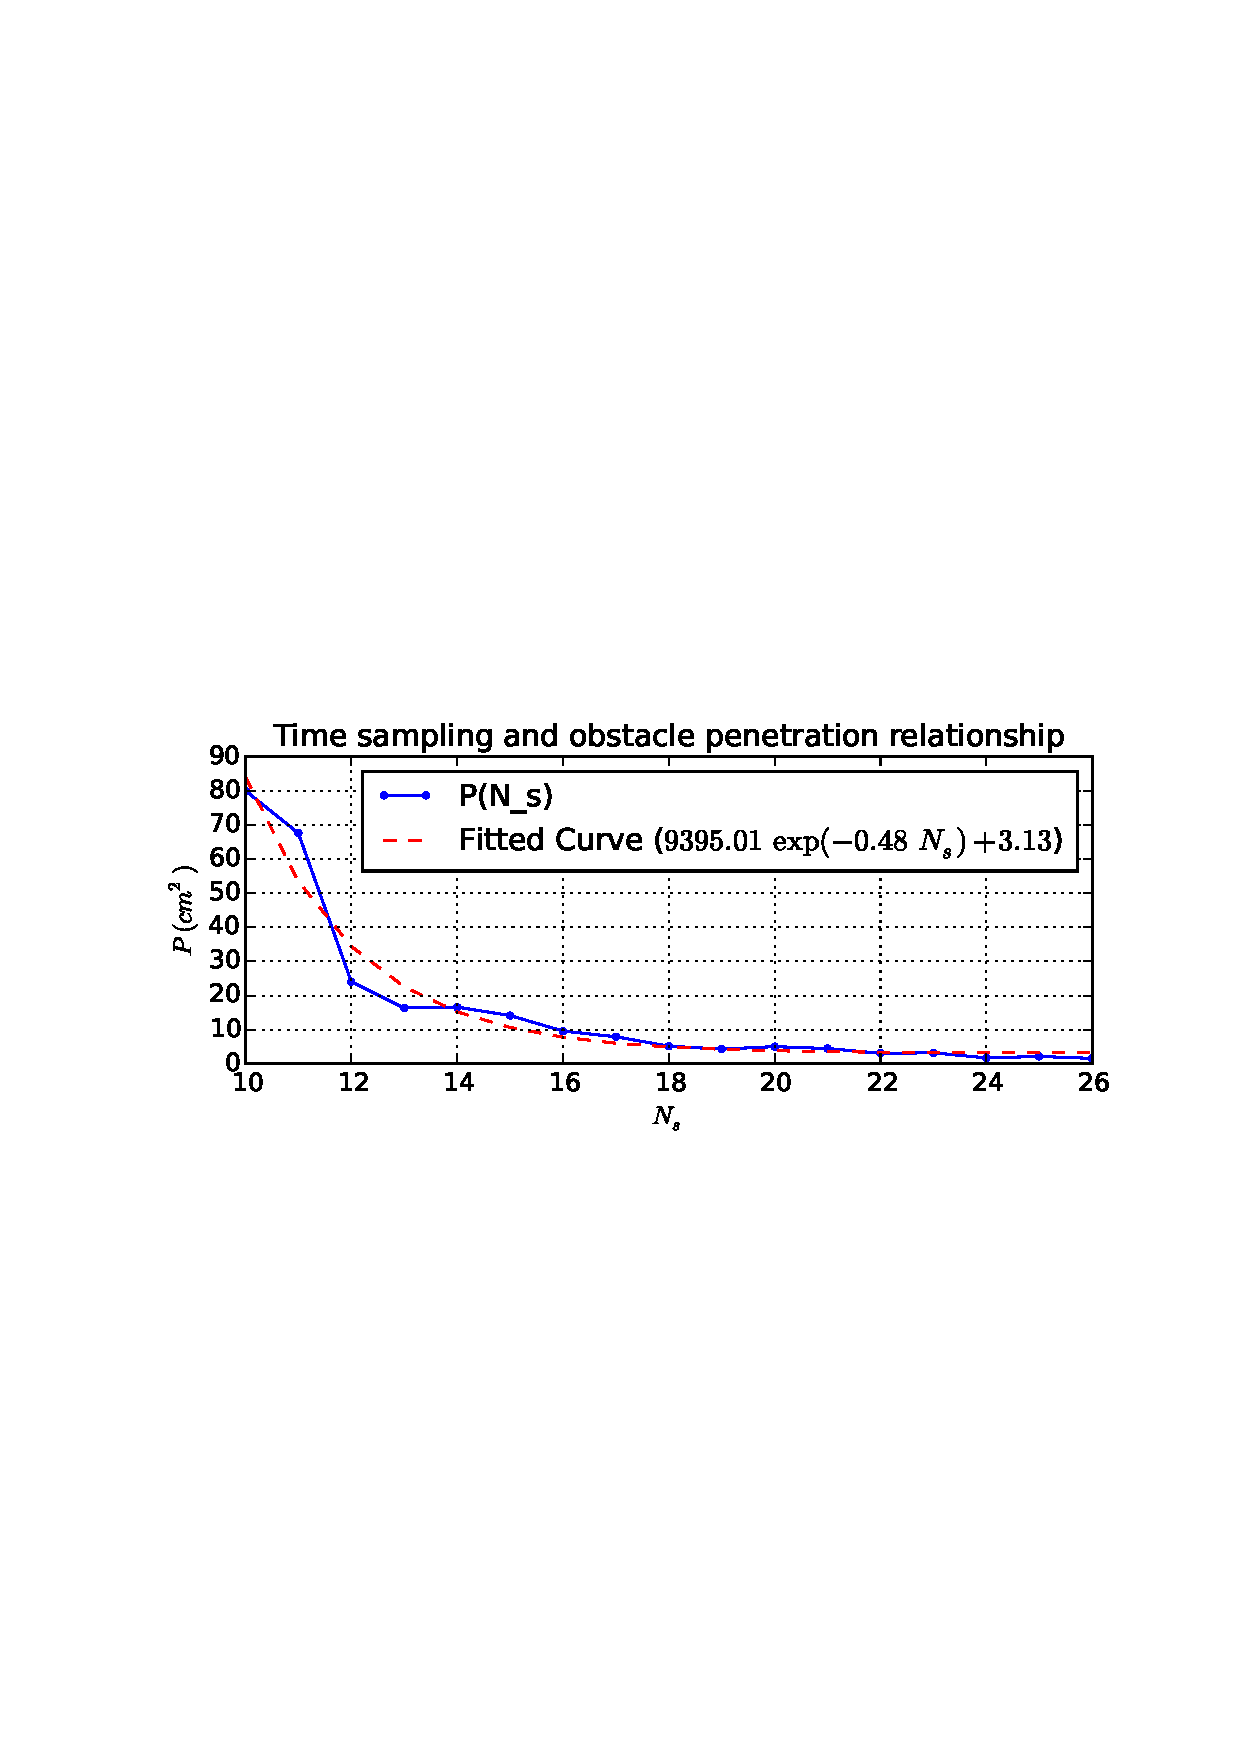
\includegraphics[width=\linewidth]{./images/penetration/pen-nsi.pdf} %
  %\rule{5cm}{5cm} % <-- this is just a black box substitute for graphics
  \caption{Obstacle penetration decreasing as sampling increases{fig:pen}}
\label{fig:res}
\end{figure}


\subsection{Total execution time $T_{tot}$}



%\subsection{Additional time for conflict handling$P$}


TODO Comparison with the other method;

TODO Before concluding do comparison with other approach and make sure to have 
multi-robot stuff

\section{Conclusions}


%\begin{nomenclature}
%\item[kg\,m^-3]{\varrho}{Liquid density}
%\item[Pa]{p}{Liquid pressure}
%\medskip
%\item{\mathit{Re}}{Reynold's number}

%\begin{acknowledgements}
%G.~Surname was supported by grant 1234567890.
%\end{acknowledgements}

TODO perspectives

Analise influence of dynamics of system, sensors, communication latency;

\bibliographystyle{actapoly}
\bibliography{biblio}

\end{document}
%kate: default-dictionary en;